\subsection{Projekt Oversigt}
I dette afsnit vises design, bruger grænseflade, implementering og test for 'ProjectList' viewet. For den fulde dokumentation henvises til Arkitektur og Design dokumentationens afsnit \ref{Design-sec:Opretbruger}.

\subsubsection{Design}
%På figur \ref{fig:ProjctListSekvens} ses sekvens diagrammet for 'Project List' viewet til Rambøll Tilsyn.
%\begin{figure}[H] % (alternativt [H])
%	\centering
%	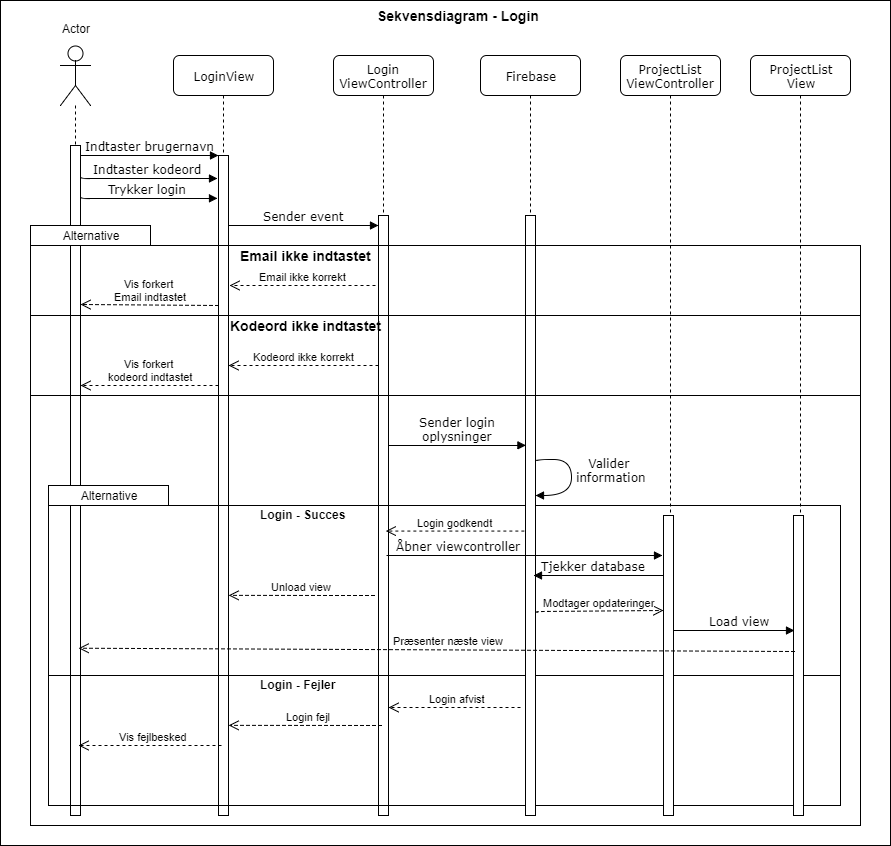
\includegraphics[height=15cm, width=15cm]{../ArkitekturDesign/Design/Login/LoginSekvensDiagram}
%	\caption{Sekvensdiagram for Login i Rambøll Tilsyn.}
%	\label{fig:ProjctListSekvens}
%\end{figure}

\clearpage

\subsubsection{Grafisk brugergrænseflade}
I ProjectListViewet er der en oversigt over hvilke projekter der ligger i databasen, samt mulighed for øverst at tilføje projekt eller tilføj bruger. Se figur \ref{fig:ProjectListView}
\begin{figure}[H] % (alternativt [H])
	\centering
	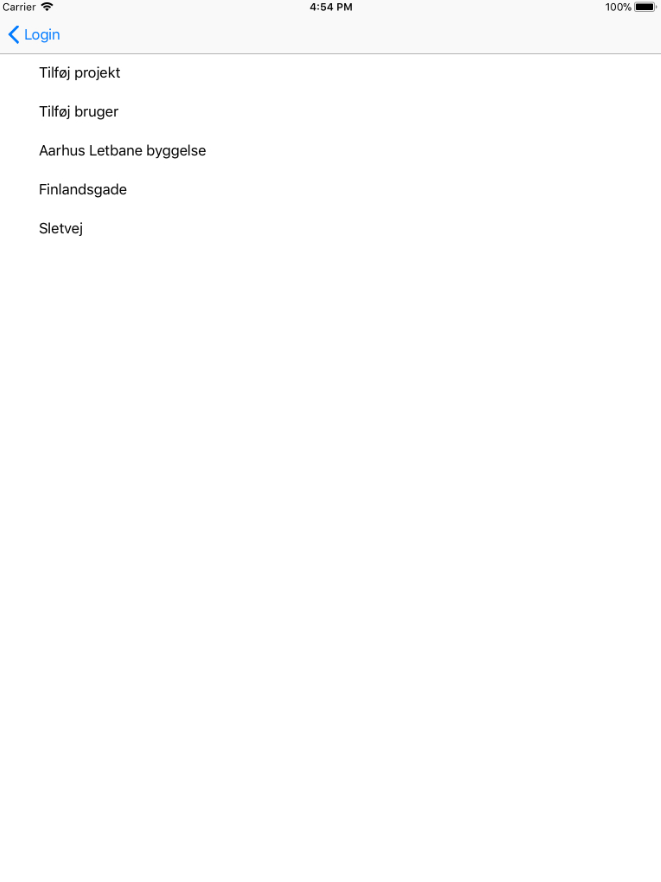
\includegraphics[height=12cm, width=10cm]{Design/Applikation/ProjektList/ProjectList}
	\caption{Login viewet som det er implementeret i Rambøll Tilsyn.}
	\label{fig:ProjectListView}
\end{figure}

\clearpage

\subsubsection{Implementering}

\subsubsection{Test}

\clearpage